% !TeX root = ../index.tex

\section{Introduction}

Architectures of modern business applications aim to be responsive, elastic and resilient.
To that end, they commonly employ the microservice pattern and message-oriented
middleware.

For certain domain or technical reasons, the communication between microservices via the asynchronous medium may require synchronous semantics.
While some works in the professional literature \parencites{millett_patterns_2015,richardson_microservices_2019,stopford_designing_2018}\todo{add more} make reference for implementing synchronous semantics in asynchronous systems, none of them go into detail.
The academic world as well does not provide a detailed examination of this topic.

The goal of this work is to create a generic concept for implementing synchronous semantics via an asynchronous medium that fulfills the requirements of being responsive, elastic and resilient.

To that end, the work follows the design science research process outlined in \parencite{cole_being_2005}.
After section \ref{sec:foundations} establishes necessary theoretical foundations, section \ref{sec:problem} examines the problem space in greater detail.
Then, section \ref{sec:method} provides a discussion of the method chosen to approach the problem described before.
Section \ref{sec:concept} derives a concept to address the problem, which is then evaluated in section \ref{sec:evaluation}.
Lastly, section \ref{sec:conclusion} discusses the results and concludes with an outlook on further work.

\section{Foundations}\label{sec:foundations}

\subsection{Reactive Information Systems}

\subsection{Microservice Architecture}

\subsection{Message-based Communication}

\section{Distributed Business Processes In Reactive Information Systems}\label{sec:problem}

This section examines the architecture of a hypothetical \gls{is} that implements a simplified version of the \gls{p2p} process.
The process describes the procurement of a company and is commonly implemented by \gls{erp} systems.
By taking an \gls{is} that implements this commonplace process as a basis for this work, the results should be easily transferable to other \gls{is} that implement other business processes.\todo{maybe remove this}

\subsection{The \acrlong{p2p} Process}

\begin{figure}[H]
  \centering
  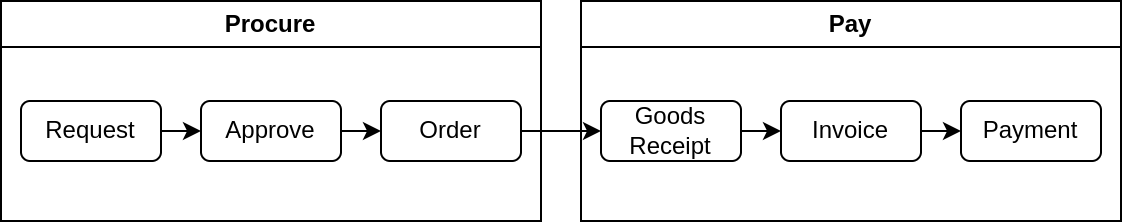
\includegraphics[width=0.9\textwidth]{procure-to-pay.drawio.png}
  \caption{The Procure-to-Pay Process}\label{fig:procure-to-pay}
\end{figure}

Figure \ref{fig:procure-to-pay} shows the distinct steps of the \gls{p2p} process.
On the procurement side, the process begins with a request.
For example, when an employee of a company requests a new stack of printing paper.
In this form of the process every request needs to be approved by a supervisor---a cost center manager for example.
An approved request can then be turned into an order by the company's purchasing department.
The order is then sent to the supplier.

When the ordered goods are delivered to the company, the process continues on the payment side.
The goods are inspected and a goods receipt is created which is checked against the supplier's invoice.
If everything is in order, payment is made to the supplier.

To be as concise as possible, the sample \gls{is} architecture described by the following only includes the procurement part of the \gls{p2p} process.

\subsection{A Reactive Procurement Application}

Figure \ref{fig:example-architecture} shows the architecture of a reactive \gls{is} that implements the procurement part of the \gls{p2p} process.
The procurement domain is decomposed into three bounded contexts: Request, Order and Workflow.
Each sub-domain is implemented by a dedicated microservice.

The \gls{ui} consists of a set of web-applications accessed by users via their internet browser.
These \glspl{ui} are not strictly separated by bounded context, but rather by use case with the aim of providing a superior user experience.
For example, purchaser's may need to edit an employee's request to correct descriptions and prices, because the employee's initial inputs were insufficient.

The microservices communicate asynchronously via a \gls{mom} with each other.
They read and write events to and from domain-specific topics within the \gls{mom}.
\todo{actually read ddd to make sure that you your these terms correctly}
\todo{explain rudimentary ddd together with microservices}

\begin{figure}[H]
  \centering
  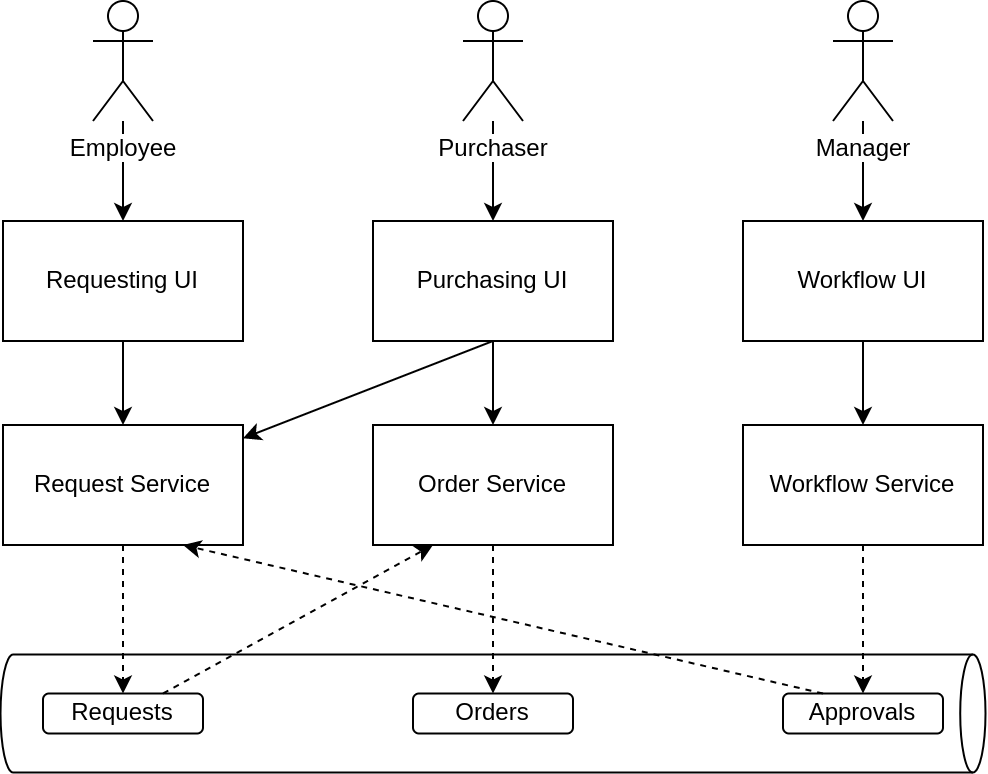
\includegraphics[width=0.9\textwidth]{architecture.drawio.png}
  \caption{The Example Architecture}\label{fig:example-architecture}
\end{figure}

In figure \ref{fig:example-architecture}, the different actors that interact with the \gls{is} in the context of the procurement process are shown at the top.
They interact with the system via the \gls{ui} fragments shown below as indicated by the arrows.
The fragments in turn interact with the microservices as indicated by the arrows.
Employees can request goods via the \emph{Requesting UI}.
Purchasers can edit requests and create orders via the \emph{Purchasing UI}.
Hence, the \emph{Purchasing UI} interacts with both the \emph{Request Service} and the \emph{Order Service}.
Requests are approved by managers via the \emph{Workflow UI} that interacts with the underlying \emph{Workflow Service}.
Although they are omitted in the diagram, each microservice is assumed to have a dedicated persistent storage.

The asynchronous communication of the microservices via the \gls{mom} is shown in figure \ref{fig:example-architecture} via the dashed arrows.
The \emph{Request Service} publishes events to the \emph{Requests} topic.
These events---in sum---contain all the information on all requests that exist in the system.
Therefore, the \emph{Order Service} replicates the requests by consuming from the \emph{Requests} topic and aggregating the events.
When an order is created via the \emph{Order Service}, it publishes an appropriate event to the \emph{Orders} topic.
From there, they could theoretically be consumed by other \glspl{is} to, for example, send them to suppliers via mail or e-mail, or to reserve a budget in the company's accounts.
Finally, the \emph{Workflow Service} publishes to the \emph{Approvals} topic when a manager approves a request.
The \emph{Request Service} consumes these events to update the status of a request when it has been approved.
This status change is then replicated to the \emph{Order Service} so that purchaser can create an order for the request.

\section{Methodology}\label{sec:method}

\section{Concept}\label{sec:concept}

\section{Evaluation}\label{sec:evaluation}

\section{Conclusion}\label{sec:conclusion}
